\section{FESDModelv2 Results}

Similar to FESDModelv1, FESDModelv2 was first trained on 64x64 pixels input images and subsequently on 200x200 pixels images.

\subsection{Results for low-resolution images}

The results of the testing after 50 epochs of training for FESDModelv2 on low-resolution images as listed in Table \ref{tab:res_v2}.

The results of the Body Part and Joint problem set have been omitted since the low resolution of the input images prohibited reasonable training for the datasets.

\begin{center}    
\begin{table}[!htbp]
  \caption[Test Results of FESDModelv1]{The test results of FESDModelv1 after 50 epochs of training.}
  \label{tab:res_v1}
  \begin{tabular}{lrrrrr}
    \hline
    {} &  Percentage of positive guesses &  Accuracy &  F1-Score &  F2-Score &  Cohen's Kappa Coefficient \\
    Problem Set   &                                 &           &           &           &                            \\
    \hline
    Full Body  &                          50.417 &     0.688 &     0.458 &     0.673 &                      0.397 \\
    Half Body  &                          55.833 &     0.767 &     0.446 &     0.789 &                      0.554 \\
    Body Parts &                          79.028 &     0.779 &     0.722 &     0.842 &                      0.257 \\
    Joints     &                          70.000 &     0.892 &     0.638 &     0.918 &                      0.773 \\
    \hline
  \end{tabular}
\end{table}
\end{center}

Note that, FESDModelv2, when trained on low resolution images obtains F1 Scores of $0.22$ and $0.50$, respectively, which are not good results as a trivial model that always predicts positive values would achieve already better F1 Scores of $0.43$ and $0.60$, respectively.

\begin{figure}[htbp]
  \centering
  \begin{subfigure}[b]{0.4\linewidth}
      \centering
      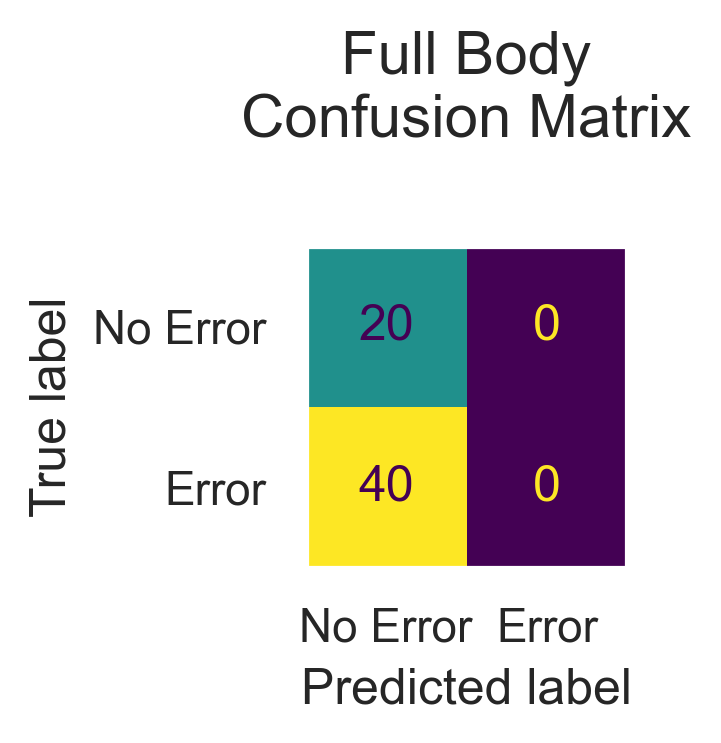
\includegraphics[width=\textwidth]{figures/Results_lo/v2/confusion/full_together.png}
      \caption[]{Full Body Problem Set}
      \label{fig:fb_conf}
  \end{subfigure}
  \hfill
  \begin{subfigure}[b]{0.4\linewidth}
      \centering
      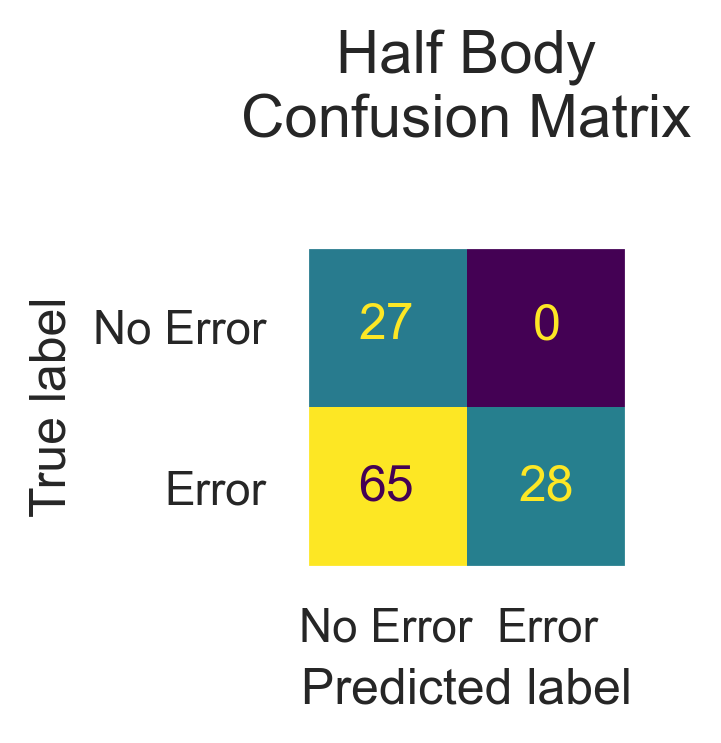
\includegraphics[width=\textwidth]{figures/Results_lo/v2/confusion/half_together.png}
      \caption{Half Body Problem Set}
      \label{fig:hb_conf}
  \end{subfigure}
  \caption[Confusion Matrices of FESDModelv2 (64x64 pixels input resolution)]{The confusion Matrices of FESDModelv2 for the Full Body and Half Body problem sets trained on input images of 64x64 pixels resolution.}
  \label{fig:conf_v2}
\end{figure}

\FloatBarrier

%
%
%
%
%
%
%
%
%
%
%
%
%
%
%

\subsection{Results for higher resolution images}

The results of the testing after 20 epochs of training for FESDModelv2 on 200x200 pixels resolution images of the Full Body, Half Body, Body Parts and Joints problem sets, respectively, as listed in Table \ref{tab:hi_res_v2}.

\begin{center}    
\begin{table}[!htbp]
  \caption[Test Results of FESDModelv1]{The test results of FESDModelv1 after 50 epochs of training.}
  \label{tab:res_v1}
  \begin{tabular}{lrrrrr}
    \hline
    {} &  Percentage of positive guesses &  Accuracy &  F1-Score &  F2-Score &  Cohen's Kappa Coefficient \\
    Problem Set   &                                 &           &           &           &                            \\
    \hline
    Full Body  &                          50.417 &     0.688 &     0.458 &     0.673 &                      0.397 \\
    Half Body  &                          55.833 &     0.767 &     0.446 &     0.789 &                      0.554 \\
    Body Parts &                          79.028 &     0.779 &     0.722 &     0.842 &                      0.257 \\
    Joints     &                          70.000 &     0.892 &     0.638 &     0.918 &                      0.773 \\
    \hline
  \end{tabular}
\end{table}
\end{center}    

FESDModelv2 achieves better F1-Score FESDModelv1 for the Joint problem set of all models when trained on images with a higher resolution. Furthermore, very promising results are achieved on the Half Body problem set with an F1-Score of 0.71. Finally, for the Full and Half Body problem sets higher F1 scores are obtained when using high resolution images.

\begin{figure}[htbp]
  \centering
  \begin{subfigure}[b]{0.35\linewidth}
      \centering
      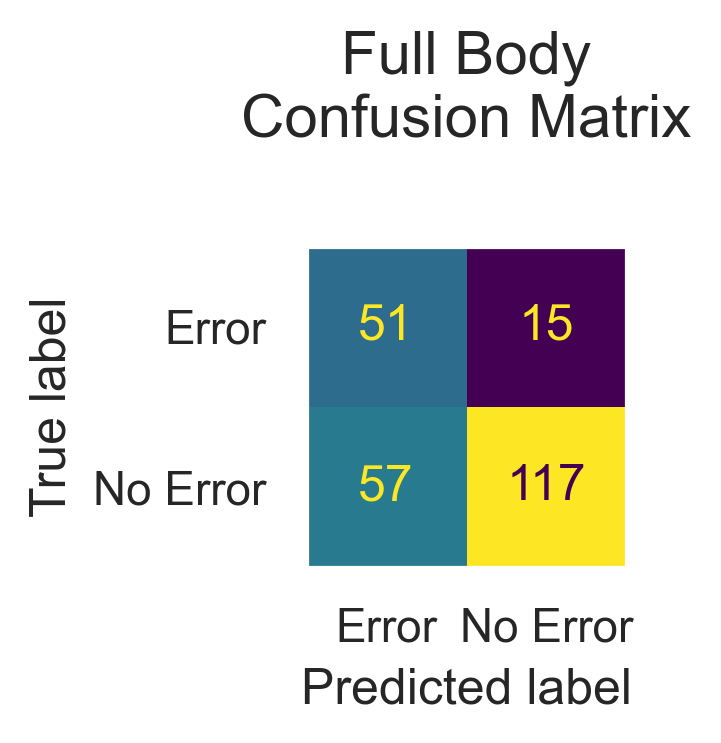
\includegraphics[width=\textwidth]{figures/results_hi/v2/confusion/full_together.png}
      \caption[]{Full Body Problem Set}
      \label{fig:hi_fb_conf}
  \end{subfigure}
  \hfill
  \begin{subfigure}[b]{0.35\linewidth}
      \centering
      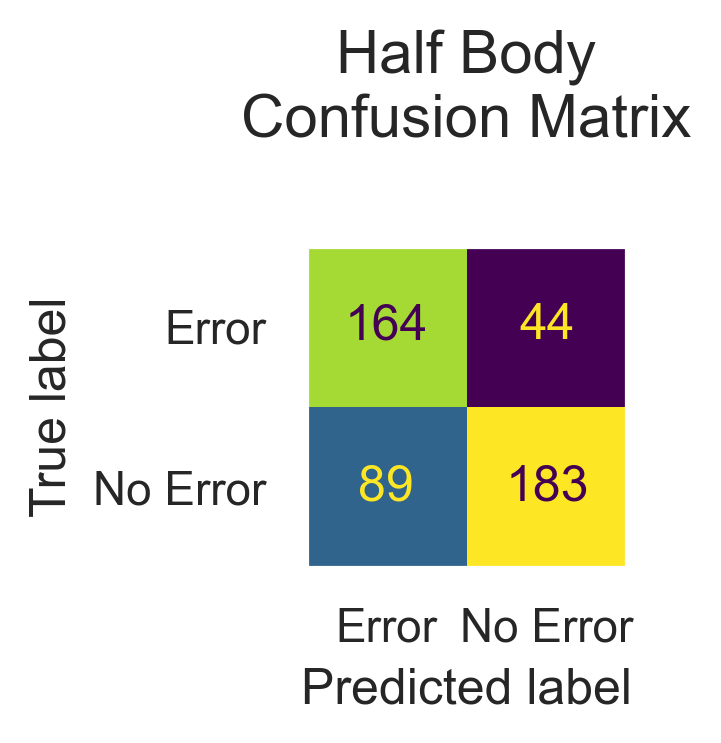
\includegraphics[width=\textwidth]{figures/results_hi/v2/confusion/half_together.png}
      \caption{Half Body Problem Set}
      \label{fig:hi_hb_conf}
  \end{subfigure}
  \hfill
  \begin{subfigure}[b]{0.35\linewidth}
      \centering
      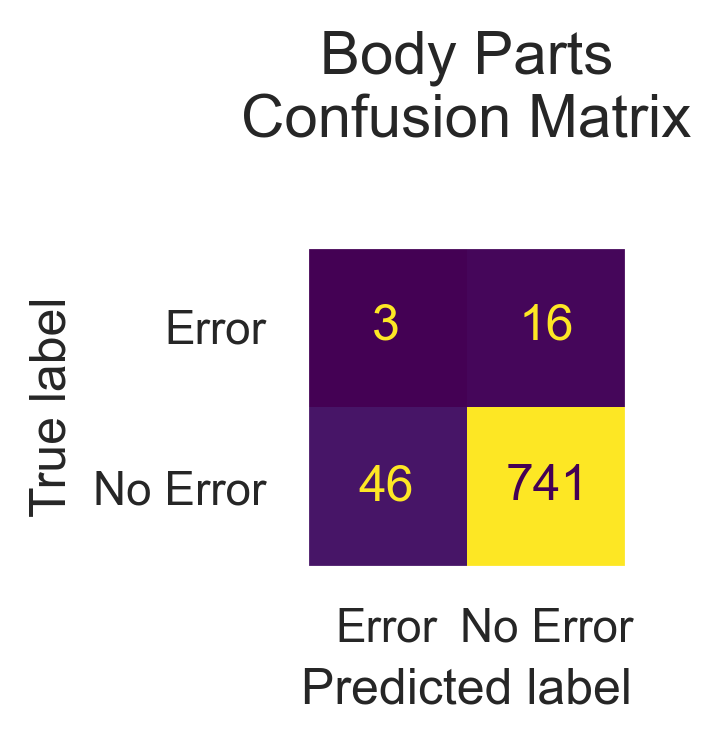
\includegraphics[width=\textwidth]{figures/results_hi/v2/confusion/body_parts_together.png}
      \caption{Body Part Problem Set}
      \label{fig:hi_bp_conf}
  \end{subfigure}
  \hfill
  \begin{subfigure}[b]{0.35\linewidth}
      \centering
      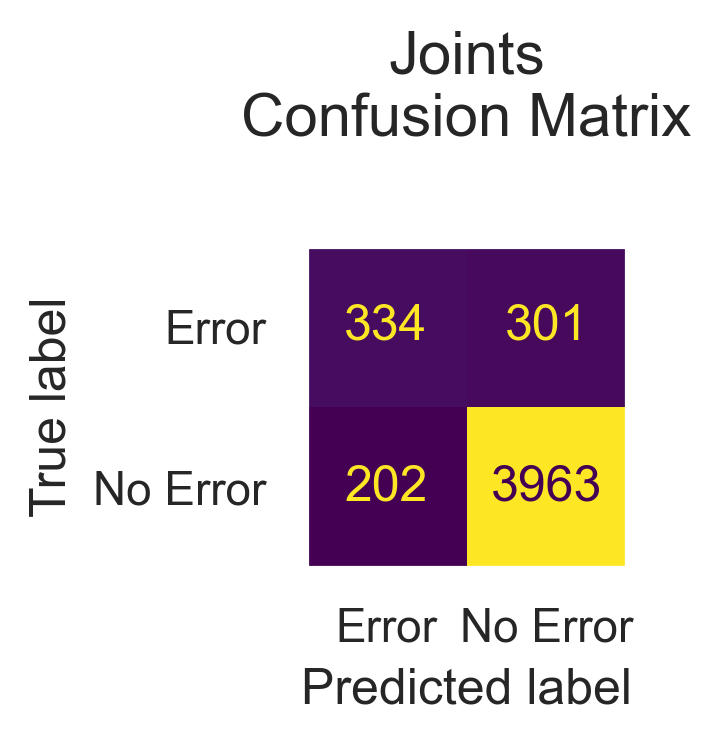
\includegraphics[width=\textwidth]{figures/results_hi/v2/confusion/joints_together.png}
      \caption{Joint Problem Set}
      \label{fig:hi_jt_conf}
  \end{subfigure}
  \caption[Confusion Matrices of FESDModelv2 (200x200 pixels input resolution)]{The confusion Matrices of FESDModelv2 for the different problem sets trained on input images of 200x200 pixels resolution.}
  \label{fig:hi_conf_v2}
\end{figure}

\FloatBarrier
